% Compile to pdf, run at command prompt:
% latex main
% makeindex main_v2.nlo -s nomencl.ist -o main_v2.nls
% bibtex main
% latex main
% latex main
% dvipdfm main.dvi
%
% tested with MiKTeX and WinEdt

\documentclass[a4paper,twoside,12pt,notitlepage,openright,12pt]{article}

% Load relevant packages
% ----------------------
\usepackage[ansinew]{inputenc}
\usepackage{graphicx} %[dvips] to used with .eps figures
\usepackage{natbib}
\usepackage{lastpage}   % page count
\usepackage{amsmath}
\usepackage{amssymb}
\usepackage[english]{babel}
\usepackage[intoc]{nomencl} % including table of content
\usepackage{ifthen}
\usepackage[hmargin=3.0cm,vmargin=3.6cm]{geometry} % setting marginals
\usepackage{fancyhdr,extramarks}  % header ja footer manipulation
\usepackage{times}  % to change font to times
%\usepackage{uarial} % as similar as Arial as possible
\usepackage{setspace} % for linespacing
\usepackage{caption}
\usepackage{booktabs}

\usepackage[ruled,vlined]{algorithm2e}
\usepackage{algpseudocode} 

% Setup ??
% --------
\newcommand{\nomunit}[1]{\renewcommand{\nomentryend}{\hspace*{\fill}#1}} % Inserts units on the right at symbol list
\renewcommand{\nomgroup}[1]{%
 \ifthenelse{\equal{#1}{C}}{\item[\textbf{Latin alphabet}]\item}{%
 \ifthenelse{\equal{#1}{G}}{\item\item[\textbf{Greek alphabet}]\item}{}}{%
 \ifthenelse{\equal{#1}{L}}{\item\item[\textbf{Subscripts}]\item}{}}{%
 \ifthenelse{\equal{#1}{H}}{\item\item[\textbf{Superscripts}]\item}{}}{%
 \ifthenelse{\equal{#1}{W}}{\item\item[\textbf{Abbreviations}]\item}{}}{}}

\singlespacing

% HEADING
% -------

\pagestyle{empty} % Alternatives: fancy, empty
\fancyhf{}% clearing the header and footer
\fancyhead[RE,RO]{\thepage}

%\renewcommand\sectionmark[1]
%{\markboth{\thesection\ #1}{}}         % section name to header
%\renewcommand\subsectionmark[1]
%{\markright{\thesubsection\ #1}}       % subsection name to header
\renewcommand{\headrulewidth}{0pt}    % ruler thickness between head and body
\renewcommand{\footrulewidth}{0pt}      % no ruler between body and footer

\setlength{\nomitemsep}{-\parsep}   % removing default extra skip between entries at nomenclature
\linespread{1.25} % Set line spacing to 1.5 https://tex.stackexchange.com/a/65985
\numberwithin{equation}{section}    % equation numbers with section numbers
\numberwithin{table}{section}       % table numbers with section numbers
\numberwithin{figure}{section}      % figure numbers with section numbers

% makeindex command needs to run at command prompt to create nomenclature list file
\makenomenclature % makeindex main_v2.nlo -s nomencl.ist -o main_v2.nls
%\bibpunct{(}{)}{;}{a}{,}{,}%


\usepackage[T1]{fontenc}
\usepackage{beramono}
\usepackage{listings}
\usepackage[usenames,dvipsnames]{xcolor}

%%
%% Python definition (c) 2014 Jubobs
%%

% Default fixed font does not support bold face
\DeclareFixedFont{\ttb}{T1}{txtt}{bx}{n}{12} % for bold
\DeclareFixedFont{\ttm}{T1}{txtt}{m}{n}{12}  % for normal

% Custom colors
\usepackage{color}
\definecolor{deepblue}{rgb}{0,0,0.5}
\definecolor{deepred}{rgb}{0.6,0,0}
\definecolor{deepgreen}{rgb}{0,0.5,0}

\newcommand\pythonstyle{\lstset{
    language=Python,
    basicstyle=\ttm,
    otherkeywords={self},             % Add keywords here
    keywordstyle=\ttb\color{deepblue},
    emph={MyClass,__init__},          % Custom highlighting
    emphstyle=\ttb\color{deepred},    % Custom highlighting style
    stringstyle=\color{deepgreen},
    frame=tb,                         % Any extra options here
    showstringspaces=false            % 
}}


% Python environment
\lstnewenvironment{python}[1][]
{
\pythonstyle
\lstset{#1}
}
{}


%%
%% Julia definition (c) 2014 Jubobs
%%
\lstdefinelanguage{Julia}%
  {morekeywords={abstract,break,case,catch,const,continue,do,else,elseif,%
      end,export,false,for,function,immutable,import,importall,if,in,%
      macro,module,otherwise,quote,return,switch,true,try,type,typealias,%
      using,while},%
   sensitive=true,%
   alsoother={$},%
   morecomment=[l]\#,%
   morecomment=[n]{\#=}{=\#},%
   morestring=[s]{"}{"},%
   morestring=[m]{'}{'},%
}[keywords,comments,strings]%

\lstset{%
    language         = Julia,
    basicstyle       = \ttfamily,
    keywordstyle     = \bfseries\color{blue},
    stringstyle      = \color{magenta},
    commentstyle     = \color{ForestGreen},
    showstringspaces = false,
}


% Actual document
% ---------------

\begin{document}

\bibliography{ref}


\thispagestyle{empty} \setlength{\parindent}{0pt}
\begin{figure}

\includegraphics[width=60mm]{./figs/Merkki_Logo_CMYK}\\
\end{figure}
~\\

\vspace{60mm}
{\sffamily\large Mikael Koli\\
\\
\MakeUppercase{\Large Building a Computational Artificial Market}}\\

%\vspace{4mm}
{\sffamily\footnotesize Thesis for the degree of Doctor of Science (Technology) to be presented with\\
due permission for public examination and criticism in the Auditorium ...\\
at Lappeenranta University of Technology, Lappeenranta, Finland on the\\
..th of March, 2011, at noon.}\\

\vspace{\stretch{1}}
{\sffamily\normalsize Acta Universitatis\\
Lappeenranta 2019}
 
\thispagestyle{plain}
\begin{center}
    \Large
    \textbf{Building a Computational Artificial Market}
        
    \vspace{0.4cm}
    \large
        
    \vspace{0.4cm}
    \textbf{Mikael Koli} \\
    July 10, 2020 % TODO
       
    \vspace{0.9cm}
    \textbf{Abstract}
\end{center}

% TODO: Purpose of the thesis is also to act as road map to build such a model
Computational economics is a branch of experimental economics that aims to 
recreate and explain dynamics of real markets using computational simulations. Researchers of
empirical economics has often very limited ability to control the market environment 
in order to studyspecific phenomena but such restrictions do not apply in pure computational
environments. The purpose of this thesis is to build a generic computational market. As the
previous literature is lacking on thorough examples of how to build such model the mechanics of this
model are discussed with detail. The model is intended to be as flexible and abstracted as possible 
while keeping the complexity of the model at minimum. The trading agents are budget constrained 
and zero intelligent in nature and the market can be described as a continuous double auction or a 
limit order book market. The model supports multi-asset simulations and the meaning of currency is 
abstracted away and any asset in the model can act as the currency or the traded asset for a market. 
The representativeness of the model is validated using stylized facts and the behaviour
of the order book is studied with various experiments.\\

The model produced similar results as the similar models from previous literature: zero-intelligent
traders do converge efficiently to an equilibrium and some of the stylized facts can be produced
with such simplistic model. Testing the model revealed several additional interesting observations.
The bid and ask sides of a generic artificial market with tick sizes are asymmetric by nature: the 
price of the bid orders are limited with the amount of currency able to be allocated to the order 
but such limitation is not prevalent with ask orders. Also, the global balance between assets in 
zero-intelligent markets is not the only factor driving the equilibrium price: also the probability 
of issuing bid and ask orders affect to the equilibrium.\\

Keywords: Computational Economics, Experimental Economics, Artificial Stock Market\\
%\addtocontents{toc}{\contentsline {section}{Abstract}{}}

\section*{Acknowledgements}

I would like to thank \{insert all\}

Thanks.\\

\vspace{\stretch{1}}
Mikael Koli\\
June 2020\\
Espoo, Finland\\

%\addtocontents{toc}{\contentsline {section}{Acknowledgments}{}}%
%\thispagestyle{empty}
\begin{center}
\vspace*{40mm}

\Large{\emph{To all of you,\\
use freely}}\\

\vspace*{30mm} \Large{\emph{Yours, JR!}}\\

\vspace{\stretch{1}}

\end{center}

\pagebreak

\cleardoublepage%
\thispagestyle{empty}%
% \addtocontents{toc}{\contentsline{section}{Contents}{}} % including contents to contents

\tableofcontents%
\listoffigures
\listoftables

\thispagestyle{empty}%
%\cleardoublepage%
\pagestyle{fancy}%

%\addcontentsline{toc}{section}{List of publications}
%\include{LOP} %List of publications


%\cleardoublepage%
\printnomenclature[2.0cm]%

\setcounter{page}{1} % Set page numbering starting from 1 from here on

% Content of the Thesis
% ---------------------

\section{Introduction}

% What's problematic with empirical research?
Due to the chaotic elements of the financial markets and lack of control, 
empirical research often face serious challenges in effort to study the 
dynamics of markets. The empirical researchers cannot control the market conditions 
and the thinking, intentions and actions of the market participants are often completely out of reach
for the researchers. The researchers may also encounter various practical challenges, such as 
lack of available data, spurious relations or changing market environment, 
which may furher limit their ability to produce robust and accurate results. 

% Solution for problems for empirics
However, the mechanics of how financial markets work are well 
understood as they are inherently artificial structures 
even though the behaviour of the market participants is not. 
The mechanics of trading exchanges are simply sets of predefined rules 
that the exchanges follow and the market clearing, the procedure 
that matches the orders and produce trades, can be described with 
deterministic algorithms. Therefore the infrastructure for trading
could be accurately recreated and used to conduct laboratory 
experiments in which the unknowns could be reduced to the market participants
themselves. Such an experiment could produce complete information about
the individual orders, formed trades and positions of each trader at any given time
and the market conditions and information available for each market participants could
be controlled in order to minimize noise or to create a desired state of the market to
study. Moreover, the impact of the market mechanics itself to the trading prices and volumes 
is possible to extract and study. 

% Why artificial markets
These experiments often complement empirical research. They aim to find the
conditions in which empirically proven phenomena may form and close the gap
between theory and empirics. 

% Types of artificial markets
Such laboratory experiments are often referred as artificial markets, or artificial
stock market (ASM). \citet{boer05} discovered three categories of artificial markets: 
experimental, computational and analytical. In experimental artificial markets human traders
are the market participants and they most often trade using a software act as
the market system. Analytical markets are simply sets of mathematical equations that
form the market mechanics. Most often however, artificial markets are associated with 
computational artificial markets. These markets are computer simulations in which 
also the roles of market participants are performed by software agents. The focus in this
thesis is on the computational artificial markets and the term is used interchangeably
with the term \textit{artificial market}. 

% Generic overview of ASM
After the first computational artificial market developed in Santa-Fe Institute
(\citet{SantaFe94}) variety of models have been developed since. Some of the
models have advanced trading agents while others aim for minimal design 
regarding to the behaviour of the traders in order to study the market
mechanics. Some studies, such as \citet{GOYKHMAN20181729}, \citet{IZUMI200535},
\citet{Reinforcement09} and \citet{YEH20102089}, use learning algorithms in the decision making of 
their agents while some, such as \citet{God93}, \citet{Jam96}, \citet{Genoa01} and \citet{Raberto05}, 
aim for minimizing the intelligence of the traders to build a market settings in which
specific attributes emerge. % TODO: Continue with 



 %Introduction
\section{Market Microstructure}

Market microstructure is the study of the mechanics in place in real markets.
It describes why trading occurs, the mechanics how trades are formed, 
how markets are organized, what information is relayed to the trading 
agents from the markets and the dynamics of price formation. \citep[p. 3-6]{Has07}
In this section we will go through various models how real markets 
are formed and what kinds of elements.

There are several common features with financial markets. They typically are
organized as double auction market 

\subsection{Double Auction}
% Call-market (Itayose, Sealed-bid) vs CDA (Zaraba)

Double auction market is widely used market structure in real 
financial markets. It is a form of auction 
in which both sides of the markets, buyers and sellers, are able to 
produce quotes \citep*{Kle99}. These quotes form the order book 
which is a collection pending bid and ask offers. A trade 
occurs between crossing and matching orders: each trade is formed between 
a bid order with a higher or equal price and an ask order with a lower 
or equal price \citep*{Ben12}. Double auctions varies in
several aspects: when the orders are matched and how the orders are matched. 
In some implementations, such as \citet*{God93}'s, a trade is 
formed only when a buyer and a seller each agree on the exact trade 
price but typically the matching of crossing orders is automated.

% \subsubsection{Order Matching in Double Auction}

Main distinction between double auction market models is when
the order matching takes place. Typically the order matching 
is continuous process occuring after arrival of each new order but
in some markets this process takes place after a specified interval
has passed, for example at the end of a trading day. \citep{boer05}
In literature, there are various terms to describe these two market models
but the mechanics are the same. \citet{boer05} used term 
\textit{call-market} for the former and \textit{continuous session market}
for the latter whereas \citet{ASt05} used terms \textit{Itayose method}
and \textit{Zaraba method} respectively to describe the same mechanics. \citet{Moc15} described
the mechanics of call-markets as \textit{periodic double auction} which
they described is an extension of a sealed-bid auction. Sealed-bid auctions
is an auction model in which the bid and ask offers
are submitted once and then the order matching is executed once. 

% More about Sealed-bid matching (supply-demand) and CDA matching

\subsection{Execution System}
% Quote-driven vs Order-driven
The execution systems are typically divided into two types:
quote-driven and order-driven. In quote-driven market the investors
trade with prices provided by dealers who are part of the market 
organization. In order-driven, the prices are formed according to
the orders submitted by the investors via automatic order matching 
or market makers. \citep{Baru17} Real markets are most often a combination
of the two \citep{boer05}.

\subsection{Price Dynamics}
% Stylized facts
The price dynamics in stock markets are known to be chaotic and hard to 
predict. The underlying elements that play a role in the price formation
are constantly evolving and it still remains relatively poorly understood.
However, there are some characteristics of price behaviour that are supported
with enough empirical evidence to be considered as properties of price in
financial markets. These statistical phenomena, called stylized facts in
econometrics, have been observed in extensive amount of studies from 
different assets, markets and time periods \citep{Shakeel18}. 
% List of Stylized facts (Cont R. (2001) & Gould et al. (2013))
Some of the common stylized facts of financial assets are \citep{StylizedFacts01} and \citep{lob13}:

\begin{enumerate}
    \item Fat-tailed distribution of returns: distribution of asset returns have fatter tails than normal distribution. Returns have positive excess kurtosis.
    \item Lack of autocorrelation: autocorrelation of returns in financial markets have shown to be statistically insignificant except in very short term. Previous return has no prediction power over the following. 
    \item Volatility clusters: volatility have measured to have positive autocorrelation. Strong price movement tend to follow additional exceptional price movements forming clusters of volatility in time.
    \item Trading volume and volatility are positively correlated.
\end{enumerate} 

\section{Computational Artificial Market}
% What is ASM, what kinds of structures they have
Artificial markets are simulation environments for analyzing, 
reproducing and gaining understanding of the dynamics of 
real markets \citep{Julien07}. However, there are several 
characteristics in real markets that cannot be replicated
in artificial setting in an obvious way. Some of these artificial
market specific issues, such as how the meaning of time is 
implemented and how the decision making of the trading agents
works, are presented in this section.


\subsection{Time Handling in ASM}

Implementing the meaning of time to an ASM is a non-trivial problem.
One may do the simple assumption that the trades occur in fixed
intervals in stock markets. This is however rarely the case in real markets
and the issue of nonsynchronous trading, also known as nontrading, emerges. 
For instance, an asset may be traded in minute basis when there is
public information released while other times it may not be traded much at all.
There may even be days without any trade. \citep{Econometrics} 

In ASM literature time handling is typically divided into two implementations:
synchronous and asynchronous. \citet{Julien07} summarized the difference as that in synchronous
trading all the traders are given the same opportunity to make their placements
while in asynchronous trading the simulation engine gives the traders the opportunity to
make decisions in disorganized manner, possibly by picking traders randomly.
\citet{Ben17} argued the difference to be more about discrete versus continuous time handling.
According to them, synchronous trading takes place in fixed time intervals whereas in 
asynchronous trading the order submission can occur in any point in time. Unarguably, 
asynchronous trading is more realistic as time is in fact continuous and traders make
their decisions in their individual frequencies.

% TODO: How this goes in this thesis?

\subsection{Trading Agents}
\label{section:ASMTradingAgents}
% TODO: Human traders?

There are multitude types of trading agents used in ASM models with varying degree
of rationality. Some models use as simplistic agents as possible to implement as
little complexity to the model as possible while some try to emulate rational 
markets with more advanced but complex traders. The most simplistic trading agents
used in the literature are traders that submit random orders. Such traders
lack the ability to do informed and rational decisions hence they are often called
zero-intelligent traders. On the other end of the spectrum, there are traders
that use artificial intelligence (AI) in their decision making. The models using
more advanced trading agents are often referred as \emph{agent-based computational
economics} (ACE).

% ZI traders
Term zero-intelligent (ZI) traders was initially introduced by \citet{God93}. Zero-intelligent
traders do not aim for maximizing profit or any other function and they do not 
possess the abilities to remember or to learn. Zero-intelligent traders are also unable
to manage risks, balance portfolio or speculate. The limit prices they submit are
often drawn either from a uniform distribution with a specified range (\citet{God93}, \citet{Mil08}) 
or from normal distribution with a mean of the last market price or the
best price of opposite book (\citet{LIU20082535}, \citet{Genoa01}). ASM models using
zero-intelligent traders are discussed with more detail in literature review. 

% ACE
\citet{LeBranon2000} argumented that the design decision on more advanced traders 
lies in whether the traders should be evolving or learning. However, the literature
generally does not make clear distinction between the terms and the term \emph{learning}
is often used to describe also evolving models. An extensive review of ACE literature 
is presented by \citet{ACE12}.

% Evolutionary
In evolutionary models the agents converge to the optimal strategy using evolutionary algorithms, typically
genetic algorithms or genetic programming. Evolutionary models are characterized by 
mutation and selection mechanics: sets of parameters for the model are created 
using random mutation between the best performing sets of parameters from last 
round, ie. trading session. The worst performing sets of parameters are discarded.
\citet{GenAlgASM18} and \citet{GenAlgBTCASM19} used genetic algorithm to select 
best performing strategies from a set of predefined trading rules. The predefined
rules were combined to form strategies using random mutation. \citet{FieldGA05} developed
similar model except instead of rules defined by the researchers they derived the rules 
by interviewing actual traders. \citet{LeBranon2001} combined an evolutionary model with a 
learning algorithm: the trading rules used in the evolutionary model were formed using a 
simple feed-forward neural network.

% Learning
Learning ASM models use machine learning for the agents to adopt the optimal strategies.
However, such models are somewhat rarer in the literature than evolutionary
models. \citet{Reinforcement09} used reinforcement 
learning, more specifically Q-learning, to predict the fundamental value of a 
dividend paying stock and this prediction was used in the agents' 
decision making: if the predicted fundamental value is smaller than the market price
the trader will sell the stock and if it is higher the trader will buy it. They 
also tested the model with an evolutionary selection to replace worst performing
traders with best performing.

% Another example of evolutionary: \citet{CHEN2001363} 
% There seems to be no pure machine learning agents even though topic mentioned in 
% LeBranon2000 and Chen S. et al (2012) Agent-based economic models and econometrics
% Used search words: 
%   Agent based computational economics & (machine learning | neural network)
%   artificial stock market & (machine learning | neural network)

% TODO: Heterogenous vs Homogenous traders

ACE models are generally specific and their goal is often to simulate a specific behaviour.
They also introduce higher amount of design decisions to validate and model parameters 
to tune compared to zero-intelligent agents. Due to these factors zero-intelligent traders
were chosen as the trader type in this thesis. The goal of the introduced model is to be as 
generic as possible and the focus is on the market microstructure and therefore the more 
simplistic approach is more suited.
\section{Literature Review}

Santa Fe institute's computational artificial stock 
market is considered to be one of the first of a kind. 
The focus of the simulation structure is more in the 
decision making process of the traders rather than in the 
market's microstructure. The model's traders use 
genetic algorithm to form a pool of rules to follow
in their decision making process. The traders can buy or
sell either risk free bond or risky dividend yielding stock.
The market is quote-driven in a sense that the traders
either accept the current price set up by the clearing house
or do not trade. The price goes up in case of there is excess
demand and vice versa. (\citeauthor{SantaFe94}, \citeyear{SantaFe94} 
and \citeauthor{SantaFe99}, \citeyear{SantaFe99})

Since then there have been many more models being 
developed with various complexities. These models are often developed
for achieving specific properties of a real market, 
usually related to the price formation. In this section
go through recent literature to describe some of the models
that has been built and discuss the design decisions in them.


\citep{Ben12}

\subsection{Zero Intelligent Markets}

\subsubsection{Gode's and Sunder's Market}
\citet{God93} observed market efficiency in a market setting
of minimal intelligence. They conducted a partly human and partly
computational laboratory experiment to replicate the market
efficiency of human traders with least intelligent computational
trading agents. \\

Their market is organized as a double auction with several
specifications. The market is continuous in a sense that the 
orders are continuously matched even though the trading was
conducted in speicified sessions. The traders were divided 
into buyers and sellers. Buyers profits were tied to their 
individual redemption values that are gained at the end of
each trading session for each bough unit and sellers' profits
were tied to their individual cost of unit. Redemption values
represent the demand function of each buyer and cost of units 
the supply function of each seller for each session. The
traders were allowed to submit orders with size of one unit
and the trade price was taken from the price stated in the 
first of the crossing orders. \\

The computational trading agents were zero intelligent traders 
who trade at random price from a predefined range. 
The first simulation was run with budget constrain: only the bids
under the redemption value and the asks over the cost of unit 
were allowed. The second simulation was run without such limitation.
These simulations were compared with the data from human traders. \\

\citeauthor{God93} found that the budget constrain is enough to 
achieve market efficiency very close to human traders. Their findings
suggest that intelligence does not to play critical role in terms of 
how to build an efficient artificial market. The more important aspect
is the characteristics of the market, not the traders. \\


\subsubsection{Jamal's and Sunder's Market}
% Continuation study from Jamal & Sunder
\citet{Jam96} expanded \citeauthor{God93}'s work and added behavioural 
elements to similar market structure. They tested the rationality of
a market with three different trader populations: bayesian, empirical
bayesian and heuristical traders. Bayesian and empirical bayesian acted
as baselines for the market rationality and the heuristical traders were
the treatment populations for which the researchers added elements of behavioural
biases: representativeness bias and anchor-and-adjust. \\

The traders in all of the populations were zero intelligent in terms of the
prices they bid and ask. Most notable difference to \citet{God93}'s market
is that instead of redemption value and cost of units determining the
supply and demand values, \citeauthor{Jam96} used private dividend payouts 
to act as such. The dividend payout is random but traders are informed
about two possible dividends. There is also an imperfect signal that the
traders can utilize to determine which of the payouts is more probable. \\

\citeauthor{Jam96} concluded that the rationality of their markets were
not caused by the rationality of the investors but the market structure.
The implemented beharioural biases in the heuristic traders were not enough 
to steer the double auction market away from the bayesian equilibrium.
They highlight the role of the market microstructure in the rationality 
of the artificial markets. \\

\subsubsection{Raberto's and Cincotti's Market}
% Another example of Intelligence vs Structure
\citet{Raberto05} experimented with ZI investors in market setting
where each computational traders can submit bid and ask offers. Their
market was also a continuous double auction which has realistic order
book setup. In their market, the traders issue random bid and ask limit
orders with a price that follows normal distribution. The mean of this 
normal distribution is the best price of the opposite book and the 
standard deviation is constant in the first experiment and linearly 
dependent on the volatility of the stock in the second experiment. The
traders do have a budget constrain. \\

\citeauthor{Raberto05} found that the fat tailed returns observed in
real stock markets can be achieved in artificial settings using limit 
order book in the price formation and it is not consequence of clearing 
house mechanism itself. They also found that volatility clusters can
be achieved with a simple dependency on the volatility. Their paper
is furher evidence that the market microstructure may be more
important than the complexity of the traders in effort to replicate
many of the properties of real markets.

% Counter Argument for usefullness of ZI
\subsubsection{Counter Argument against ZI markets}
\citet{Mil08} provided counter argument on the usefullness of zero
intelligent traders. They replicated market structure from
\citeauthor{God93}'s study with one major difference: how the 
time is handled. In their market version, the demand varies
also between sessions and buyers can plan for it by buying units
in advance for periods of higher demand. Unlike human traders,
zero intelligent traders obviously cannot plan ahead and a market
populated with such traders cannot gain allocative efficiency comparable
to a market populated with human traders. 


\subsection{Generic ASM Frameworks}

Most of the literature in the field of artificial stock markets 
focus on recreating phenomena from real markets in artificial settings
and often these studies are lacking in details of how the model was created.
They may include descriptions how the clearing is done or how the trading agents 
come up with their decisions but usually they do not discuss about practical matters 
such as how the interactions between the simulation components work, where the 
information about traders' positions are stored or how the simulation is orchestrated. 
Studies that describe how to actually build a realistic computational 
market are quite rare. In this section discuss about some of the generic
frameworks designed in the field in order to illustrate how to structure the computational
environment.


\subsubsection{Object Oriented ASM}
% Gaia
\citet{Ben12} developed a realistic but abstract artificial stock market
model for continuous double auction using a modeling methodology known as 
Gaia. Gaia is a software design methodology for agent-based systems which 
highlights identifying the roles of the system and interactions in between.
The final model the researchers came up with is an object oriented 
approach consisting of five roles: a market, traders, a company, banks
and external world. The roles of the market and the traders in the model 
are rather similar as discussed already in this thesis. Interestingly,
even though banks and companies are identified as separate agents, 
the amount of cash and stocks are tracked in the trader agents themselves.
They, however, do not have permission to update their wealth independently. 
Banks and companies, on the other hand, act as middlewares for informing 
traders when and how much to update the amount cash and stocks. Banks also pay 
fixed interest based on the amount of cash each trader holds and companies 
pay dividend for each share. External world is a container of exogenous 
information, such as paid dividends or news, that can be used by the traders for 
their decision making. The researchers also discussed that the model could be
simplfied to only trading agents and market agent by including banks', companies' 
and extrnal world's roles to the trader agents in case of less complex but 
less detailed model is required.

The orders in their model requires the following information to be valid:
stock name, time-stamp, volume and the quoted price. These orders are stored
in the market's order book, in case they cannot be immediately matched, but 
also in the trader agents themselves for possible cancelling purposes.

% Something about the interaction model and order matching

As they did not build a working software using the model, it is unclear
how practical the model is and how easy it is to program. The model, 
however, is detailed and served as an inspiration in this thesis even though
its structure and design decisions were not strictly followed.


\subsubsection{ASM with a Concrete Implementation}
% Testing double auction as a component within a generic market model architecture
\citet{Julien07} built a simpler abstract representation of an ASM consisting
only of the trading agents, market and external world. On top of this model, 
they also created a more detailed concrete framework which they tested with
zero intelligent traders and asynchronous continuous double auction as market
model. The framework is modular in a way that it allows heterogenous traders
that emit and accept different amount of information to live in the same 
simulation environment. The researchers used translators in between the 
trading agents and the market in order to transform the orders submitted by
the trader agents and the information emitted by the market to a unified format.
For example, in case a submitted order had only the direction and the quantity 
defined, the translator fulfills the order price with the current market price 
transforming the order essentially as market order. The framework also had a
unit called simulation engine to handle the interactions between the components.

The flow of the system consisted of six steps which can be summarized with three:
\begin{enumerate}
    \item The simulation engine let all or some of the trading agents submit their orders 
            using the exogenous information provided by the external world and 
            information about the balance between supply and demand provided by the market.
    \item The simulation engine commands the market to clear.
    \item The simulation engine commands external world to update its information.
\end{enumerate}


\begin{figure}
    \includegraphics[width=\linewidth]{diagrams/julien_market.png}
    \caption{Framework defined by Derveeuw et al. (2007)}
    %\label{fig:boat1}
\end{figure}

% Something to wrap up like where the positions are saved?

\section{Methodology}

As discussed, the market type for the artifical market was chosen 
to be continuous double auction or more specifically limit order market.
The artificial stock market created in this thesis was written in Julia
programming language and it took inspiration from previous literature.
The literature is lacking on practical studies about how to actually create
an artifical stock market and therefore the actual structure of the market is explained
in depth. The decisions about the microstructure and the trader behaviour
is most closely to the work of \citet{Genoa01} and \citet{Raberto05}
whereas for the structure and practical implementation the inspiration
was taken from the work of \citet{Ben12}. The goal was to create a generic artificial market 
model with empahsis on flexibility and practicality. Many of the features
of the model are not tested in this thesis because of the scope of the thesis.
The plotting and analysis of the results were conducted using Python and its scientific
computing stack including Numpy, Pandas, Statsmodels, Matplotlib, Seaborn and Scipy library.
In this section the rationale for the programming choice of the model is discussed
and the model structure, mechanics and generic characteristics are 
explained.

\subsection{Julia Language}
Julia is relatively new dynamic programming language, 
reaching stable release of 1.0 in August 2018 \citep{JuliaV1}.
It is a performant language with an empahsis
on productivity. Even though Julia has a focus on scientific 
computing it considered as a general-purpose programming
language. Some of its features include
multiple dispatch, just-in-time compilation and built-in
matrix data types \citep{Julia}.

Julia fits well in building an artificial market.
Artificial markets can be seen as sets of objects
and interactions in between, as described \citet{Ben12},
and in such models object-oriented programming (OOP)
is preferred. Even though Julia is more functional in nature, 
features of OOP could be constructed with Julia's mutable structs 
and type annotated functions. Also, the speed of code execution, 
support for matrix operations and good productivity makes 
it viable language for prototyping simulation systems. 


\subsection{Generic Structure of the Model}
% Describe the generic structure (Type hierarchy, layers etc.)
% Kind of the static side of the simulation
The ASM model has three layers: abstraction layer, concrete 
layer and simulation layer. The fist layer, abstraction layer, contains the 
generic parts of the framework that are independent and obvious in terms
of functionality. For example, how to get traders' positions, how to
transfer assets from a trader to another or how to cancel an order are
functionalities that are independent on the type of the traders 
and type of the markets, and therefore these functionalities have little
far-reaching decisions to make. The main purpose of this layer
is to separate generic and obvious functionality from blocks of code
that has more degrees of freedom and less obvious design decisions to make.

The second layer, the concrete layer, defines the actual types and the
functionalities that require less clear and more heuristic
approach than the abstract layer. This layer also includes significant
portion of choices to make. Some of the components
on this layer include the zero intelligent trader and the
functions that defines its behaviour, the continuous double auction
market and the functions for its price formation mechanics.

The third layer, simulation layer, manages the simulation as a whole.
This layer defines the ecosystem where the simulation takes place including
the initiation of the components, iterating over the time periods, asking
each trader to make their decisions and ask the market to clear. 
Also, initial conditions including the number of sessions, investors, assets and markets
and the amount of each asset each investor owns are defined here. 
This layer mostly calls the functionalities created in the lower layers.



\subsection{Simulation Process}
% Describe how it works, how the dynamics flow etc.
In functional sense, the model consists of three main components:
the main level code, traders and markets. The main level code 
orchestrates the flow of the simulation while traders and markets
handle the pieces of functionalities associated with them. The process
is generalized in ~\ref{fig:sim_proc}. The beginning and the end of the 
simulation are shown in orange in the figure. Yellow boxes represent
the actions that belongs to the concrete layers and all the actions that
are in the main are part of the simulation layer. The remaining belongs
generally to the abstract layer.


\begin{figure}
    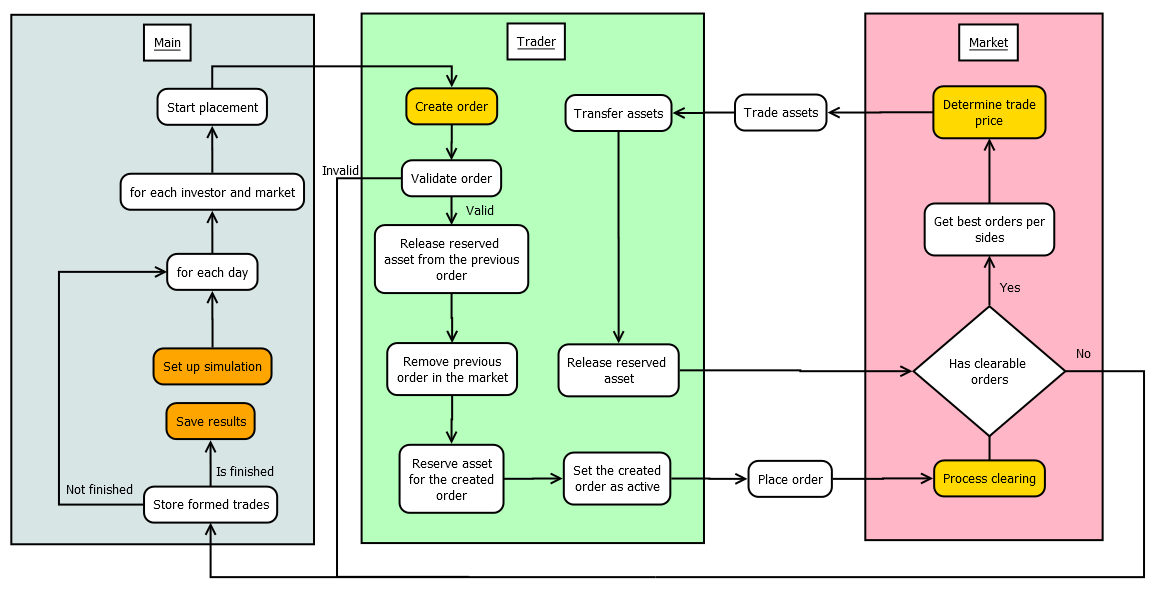
\includegraphics[width=\linewidth]{diagrams/placement_clearing_process.png}
    \caption{Simulation process}
    \label{fig:sim_proc}
\end{figure}

The simulation begins with setting up the parameters such as number of
trading days and initializing the traders, their assets and the markets.
Then each trading session is iterated in which each trader can create order 
an order to each market. After the order creation the order is validated.
The traders have also an option not to create an order. If the order was
valid, the previous order to the market is cancelled and the needed 
asset is reserved for the order in case it executes. The asset
reservation is to prevent traders going over with their budgets if they
have allocated the same asset in other markets. Next the order is
placed to the market and the clearing process begins in case of 
continuous double auction market. If there are any clearable orders,
they are traded with a price defined by the market type. When
all clearable orders are cleared, the code execution returns to the
main block and either next trading session is started or the next
trader gets a chance to make orders. In this section, the process how the
zero intelligent traders conduct their decisions and how the 
market price formation and clearing works is discussed with more detail.
There are some interesting characteristics in the asset dynamics of this
artificial market and these are also discussed.

\subsubsection{Trader Behaviour}
% How the investors make decisions actually

As mentioned, the traders of the ASM model are zero-intelligent
traders. The reason for this is to minimize the degrees of freedom introduced with
the model and provide as generic structure as possible. The traders' rationality 
for making decisions is reduced to minimum effectively making them unable to speculate, 
manage risks or optimize portfolio. They do not possess ability to seek profit, 
observe the markets or learn from their previous actions or peers and
they are only able to submit random orders. The mechanics of zero-intelligent traders
are implemented in a way that they are given sets of allowed ranges 
and options in which they choose values randomly. This way the zero-intelligent behaviour is maintained
in addition to have similar options that there are present in real markets 
concerning to order placement such as the order quantity, order price and whether
to submit an ask order, a bid order or do nothing. The traders are also budget constrained
in order to achieve allocative efficiency as proposed by
\citet{God93}. Budget constrain prevents short selling or borrowing any asset.


An order placement decision in the model requires three components 
to be defined by a trader: order side, order quantity and order price. 
There are obviously two possible sides of an order: bid and ask, but
not submitting an order is also a choice. Therefore, the traders
have three options: submitting bid limit order, submitting ask limit order
and not submitting an order. Submitting an order also cancels any previous
order created by the trader to the same market but not submitting an order does not
cancel any previous orders. The traders pick one of these options randomly 
based on the weights specified in the parameters of the simulation run. 

Determining the order price and order quantity are not as straight
forward as their feasible ranges cannot be determined completely independently
from each other and the calculations of these ranges differ between bids and asks. Bid order's
value cannot exceed the amount of currency the trader possesses thus this is 
a limiting factor for both, order quantity and order price of a bid. In addition,
the maximum order quantity is inversely proportional to the order price and
therefore if order price is set first, the maximum order quantity the trader
can set for a bid equals to its amount of currency divided by the price and vice versa. 
However, ask orders do not have such restrictions: the value of an ask order
does not reflect to the amount of assets the trader allocates to sell with the order. The
price of an ask order can, in theory, be infinite and the selling trader has no issues
fulfilling the trade on its behalf even though in practice there is no buyers
able to match with such order. The only limit for the trader placing an ask is the 
amount of the traded asset it possesses: the trader cannot sell more of the asset 
than it has. To summarize, an ask order's feasible ranges for quantity and price 
can be determined independently but this is not the case for bid orders. These feasible 
ranges are shown in ~\ref{eq:feasible_ranges}.

\begin{equation}
\begin{aligned}
% Bid
p_{bid} &= \left[1, pos_{ccy} / q \right] \\
p_{ask} &= \left[1, \infty \right] \\
q_{bid} &= \left[1, pos_{ccy} / p\right] \\
q_{ask} &= \left[1, pos_{asset}\right] \\
\end{aligned}
\label{eq:feasible_ranges}
\end{equation}

To overcome this and to maintain symmetricity between the placement of bids and asks, 
the traders decide the amount of an asset to allocate with an order instead of deciding 
the order quantity directly. This decision is independent on the order price for both
sides and can be handled the same way for both cases. Therefore, a trader placing a bid order 
need to define the amount of currency to allocate with the trade and a trader placing an ask
order need to define the amount of the traded asset to allocate, the order quantity in this case. 
The order quantity for a bid is calculated after the amount of asset to allocate 
and the order price have been set. The amount of asset to allocate is drawn from a uniform
distribution in which the minimum is one and maximum is the amount of the asset the trader
has and is free for allocation. The order price is drawn from a normal distribution in which 
the mean is the last market price. The standard deviation of the distribution is set to a 
constant and the distribution is truncated between one and infinity.

% TODO: Show and discuss about the ranges of the orders

An example of the distribution of order prices and quantities
is show in ~\ref{fig:generated_orders}. The figure contains simulation
of 1 000 000 orders created by a zero-intelligent trader. 
The last market price was set to 1 000 units and the standard deviation of the price to 10. 
The trader possessed 10 000 000 units of currency and 100 000 
units of stock.

\begin{figure}
    \centering
    \begin{subfigure}{.5\textwidth}
      \centering
      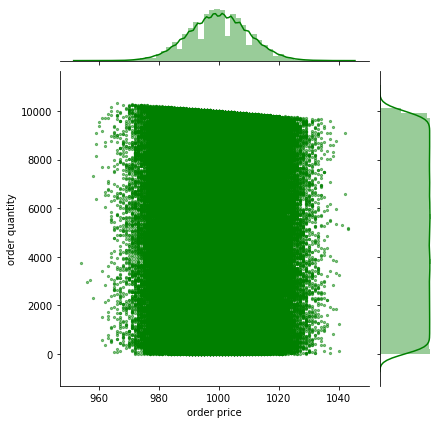
\includegraphics[width=\linewidth]{plots/order_distr_bid.png}
      \caption{Distribution of random bids}
      \label{fig:gener_bids}
    \end{subfigure}%
    \begin{subfigure}{.5\textwidth}
      \centering
      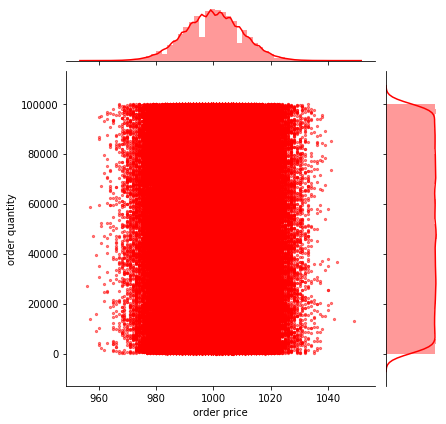
\includegraphics[width=\linewidth]{plots/order_distr_ask.png}
      \caption{Distribution of random asks}
      \label{fig:gener_asks}
    \end{subfigure}
    \caption{Distribution of random orders}
    \label{fig:generated_orders}
\end{figure}



In the literature, zero-intelligent traders are often implemented differently. For example, in the studies conducted by 
\citet{God93}, \citet{Jam96} and \citet{Mil08} the traders were initially divided to buyers and
sellers, traders could only trade one quantity of a stock per order and the prices
were drawn from uniform distribution. However, these markets did not aim for
realistic market microstructure. The trader behaviour in this model is close with the Genoa Market
created by \citet{Genoa01} as in this model the prices are also drawn from normal distribution and
the order quantities are derived from the required amount of asset. However, in Genoa Market the
normal distribution's mean is 10\% higher for ask orders and 10\% lower for bid orders from the
latest market price in order to increase liquidity. For maintaining simplicity, the mean of the distribution
is set to the last market price in this model. Also, the option of to not make an order seems not to be
implemented in the literature. However, \citet{Raberto05} implemented waiting times and order cancellation
after specified times which may produce similar behaviour. 

\subsubsection{Time Handling}

The time in the simulation took inspiration from the asynchronous model created by \citet{Julien07}. 
As in their ASM model, in this model the traders are randomly given the ability to speak and make 
their trading decisions. The proportion of traders allowed to make a decision is defined in
speak ratio which is a parameter for the simulation. After randomly selecting the traders
according to the speak ratio this set of traders is shuffled randomly and are asked to do trading 
decisions one by one for each market. However, it is unclear how the interval between placement 
decisions should be interpret in terms of real time units such as seconds or minutes. In addition, 
the issue of nontrading is also inherently present in the model: the time interval between trades 
is non-fixed.

The submitted orders and created trades include timestamps. For orders the timestamps are used
to determine the comparable age of each order. This is useful for clearing mechanics that sort 
order by their comparable age to determine the clearing price. In case of trades this information
is useful for analytical purposes to determine the timeline of events. A timestamp is simply 
an integer starting from one at the beginning of the simulation and has no additional 
intended representation. Each checking of time increments it with one unit.

\subsubsection{Market Mechanics}
% How the market is cleared actually 

The market is continuous and double auction in nature.
The clearing mechanics themselves are, however, 
rather the same as could be for a call market: 
the orders are cleared until there
are no bid orders with price equal or exceeding the
ask order with lowest price. 
Continuity is achieved by launching the clearing process
every time an order arrives to the market. 
The clearing mechanics are defined in 
the abstraction layer in a way that the same body
of code works for call markets and continuous markets
and the distinction between the markets, such as how 
the market price is formed, is handled inside the clearing
mechanics by calling the parametrized functions that are 
defined explicitly for each concrete market type. 
The main body of the clearing function, 
as written in the source code, is shown in the listing ~\ref{lst:clearing}.
In the listing, the clearing price resembles the market price
of the clearing session which is calculated for call markets but not for 
continuous markets. For continuous markets this price is simply nothing and
the price determined from a pair of crossing orders is used instead using function
\emph{get\_trade\_price}. The rationale for the complexity is that in future experiments
that study call markets could utilize the same code without modifications 
even though call markets are not studied in this thesis.

It should be noted that this mechanic may not be optimal in terms of performance: 
only the newly submitted order may possibly be cleared and therefore more 
optimized solution could utilize the fact that only this order and the opposing book
need to be compared and not necessarily the both of the books themselves. However,
in this case simplicity was considered more important than code execution speed.


\begin{lstlisting}[caption={Clearing process},label={lst:clearing}]
...
# The clearing price is defined here
# in case of call market. Nothing
# should be returned if the price
# is defined per order pair basis
clearing_price = get_trade_price(market)
while maxprice(buy_book) >= minprice(sell_book)

    order_sell = get_best(sell_book)
    order_buy = get_best(buy_book)
    
    # trade_price is clearing_price if defined,
    # else calculated per order pairs
    trade_price = (
        ~isnothing(clearing_price) ? 
        clearing_price
        : get_trade_price(order_buy, order_sell, market=market)
    )

    trade = trade!(
        order_buy, order_sell, 
        price=trade_price, 
        from=market.currency, 
        to=market.traded_asset
    )
    ...
\end{lstlisting}

The price formation of the continuous market is implemented
on the order pair basis. The trade price is simply the price
stated in the older of the paired orders. % SOURCE: find a source to describe why this way the price
The quantity of the trade is chosen from the smaller of the two orders
and the bigger order is partially cleared in case they were not 
equally sized.

% About literature


\subsubsection{Handling of Assets}
% Why use integers as units for assets

The model is constructed in a way that enables usage of multiple assets
and the assets are handled symmetrically. The former is achieved with
allowing multi-asset positions and multi-asset resersing and 
it is the simulation layer's responsibility to decide the assets, 
markets and ask the investors to create orders on them. 

Asset symmetricity means that there is no universal or central currency 
and the currencies are handled as any other asset. In theoretical sense, 
currencies are also just investment options and there is no inherent reason why other 
asset classes, such as stocks, could not operate as the definition 
of value. This feature creates complexity to the model compared to a model
with a central currency acting as the baseline for value but it also enables an
abstracted structure that handles natively cross currency
markets or ecosystems in which there exist markets between assets A and 
B and between B and C but not between A and C. This is also a better 
representation of theoretical markets.

Support for multiple assets and asset symmetricity is constructed by storing 
the owned and reserved assets of a trader to the same data structures regardless
of the type of asset in question. Each trader has one dictionary for positions
and one for reserved assets and the keys for the dictionaries are the assets.
In addition to the traded asset, markets also contains the information 
about the assets in the market. Each market has an attribute, or a field as called
in Julia, for the asset the market uses as currency to trade with and for the asset
traded in the market. As order submission occurs on market basis, this information
is used to determine what asset should be allocated for the order from the trader's
reserve and to determine the assets to exchange when a trade is formed in a market. 
The orders need not to have the information about the assets in question as orders are always
market specific in the model. This mechanic also allows interesting ecosystems in which
multiple markets can coexist that trade the same asset with using the same asset as
currency. 

% Asset allocation, reserve & active orders
% TODO: UPDATE: wording is less shit but still shit
In single market models disallowing the orders that would require more assets to execute
than there is in the trader's position should be sufficient to maintain the budget constrain. 
However, for multi-market ecosystem this is not enough. The quantities of an asset 
that are already allocated to a market via orders must be kept track of and the total amounts of 
allocated quantities must not exceed the actual asset positions of the trader. If the maximum allowed 
allocation not enforced and if there are multiple orders of a trader executing allocating same asset
there is a chance that the trader's position goes negative. 
To prevent this, this ASM model keeps track of all of the allocated assets, called reserved asset 
in the simulation, in addition to the actual asset positions. The model also
accepts only one order per trader per market as it makes little sense that
the traders are allowed to express multiple different opinions to one market 
simultaenously: especially having a bid and an ask orders on the same market
at the same time may lead to a confusing pattern where a trader is trading with
itself and therefore artificially pumping up the trading volumes. 

In addition to this, the order that a trader has already placed
to a market is tracked in the trader's data structure to make cancellation easy
but also implement relevant additional feature: active order lookup. To prevent that
the placing of a new order is not limited with the trader's existing order in the market,
the effect of this previous order, called active order, in the asset reverse is excluded. 
This active order will be cancelled as soon as this new order is validated and this new order
will become the active order thus it is not a valid reason to make the trader's placing 
options more conservative.

% Integers & bid-ask asymmetricity
All quantities of assets are stored as integers to prevent wealth leakage
or creation because of the floating point arithmetics. Using integers also
conveniently act as the tick size for all the markets. This also has the side effect
of that also all the prices must be represented as integers as one piece
of traded asset must equal exact quantity of the asset used as a currency
in the market. Furthermore, this creates deficency in the market if the quantities
of owned assets are small and a phenomenon of asymmetricity between bidders and askers
araises. The price set by an asker can be virtually anything: they can set
arbitrary positive price for their order as the only limitation is the amount
of traded asset they can commit to the order which is independent on the price. 
Every unit of increase in order price means more profit for the seller
in case the order is executed. On the otherhand, because of the 
lower limit of one in price the bidder does not have the same freedom.
The maximum price the bidder can set equals to the quantity of the asset
that behaves as currency in the market but the minimum price is one. This is
illustrated in the figure ~\ref{fig:buy_sell_asym} in which the all possible
combinations of quantities and prices are shown. The buyer owns
ten units of currency and the seller respectively owns ten units of traded stock in
this example. The colored areas represent where the possible combinations
lie.
 % And what this causes etc.
 % Price can be anything for seller but for buyer, there are boundaries

 \begin{figure}
    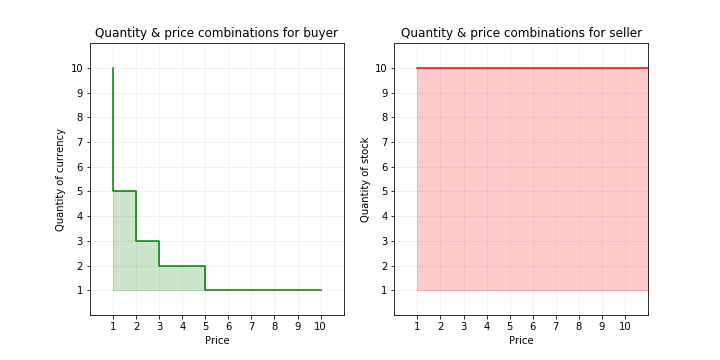
\includegraphics[width=\linewidth]{plots/buyer_seller_asymmetricity.png}
    \caption{Illustration of buyer-seller asymmetricity}
    \label{fig:buy_sell_asym}
\end{figure}

The bid-ask asymmetricity may become issue when the price of the market
approaches one. Near one the tick size start to reduce the efficiency
of the markets: for example, only one tick drop for a market price 
of four is 25\%. In addition, there may be an issue that the efficient
price cannot be reached if it lies under the price of one. Probably
the simplest solution to avoid this while still having integers for quantities 
of assets is to make sure the traded asset has sufficiently high value
compared to the currency of the market. This can be achieved simply injecting
enough currency to the ecosystem to inflate the price. Another interesting 
solution to solve the problem of the potentially unreachable efficient price 
is to have two markets for the same asset pairs but opposing direction. 
The first market trades an asset A with an asset B but the 
other market trades the asset B with the asset A. The price of the other market
should always be multiplicative inverse of the other so the.
This solution is shown in the figure ~\ref{fig:opposing_markets}. The total
amount of stock is increasing, thus inflating, and the total amount of
currency is decreasing, thus deflating, in constant rates.

\begin{figure}
    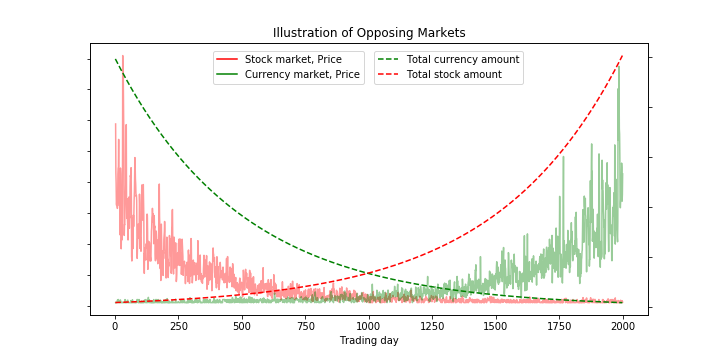
\includegraphics[width=\linewidth]{plots/opposing_markets.png}
    \caption{Two markets with inverse assets}
    \label{fig:opposing_markets}
\end{figure}


The efficient price of the market cannot be reached if it
lies below one. Therefore the simplest solution to the problem probably
is to make sure that the price of the traded asset is never close to one
To avoid any side effects from the bid-ask asymmetricity, there are two solutions:
either have two opposing markets for same asset pairs or have a balance between the 
assets in a way that orders with a price of one are unlikely. 
% implmenentation of payoffs (dividend, interests etc)

% How the literature
%Most of the ASM literature study only ecosystems in which
%the traders can only trade a stock with a cash.
% References
% ----------
\renewcommand{\thepage}{} % Stop page numbering in references
%\def\refname{what ever}% to change References title
\addcontentsline{toc}{section}{References}%

\fancyhead[LO]{\nouppercase{\bfseries\firstleftxmark}}%
\fancyhead[RE]{\nouppercase{\bfseries\lastrightxmark}}%
%\bibliography{ref}%
\bibliographystyle{LUTapa2}
\extramarks{}{References}   % this will remove the "References" to be appearing at the header at first page of bibliography
\extramarks{References}{References}

%\bibliographystyle{LUTapa}%

%\bibliographystyle{LUTapa1}% %This won't shorten 4 or more author to "et al." in reference list


%\cleardoublepage %

\end{document}
